\section{Einleitung}
Zur Umsetzung des Tools wurde das Projekt in verschiedene Arbeitspakete zerlegt, wobei jedes Arbeitspaket auf den Vorgänger aufbaut. Diese Arbeitspakete und die damit verbundenen Herausforderungen werden nun erläutert.

  
\section{Arbeitspakete}
\subsection{Traversierung aller relevanten Dateien} 
Softwareprojekte bestehen aus Hunderten von Dateien, die nicht alle Quellcode enthalten. Beispielsweise gehören Konfigurationsdateien, Ressourcedateien wie Bilder oder binäre Dateien zu den Dateien, bei denen eine Analyse der Softwaredokumentation nicht zweckmäßig wäre oder sogar zu Fehlern führen könnte. Daher ist es sinnvoll, bestimmte Dateien bei der Analyse auszuschließen beziehungsweise nur bestimmte Dateien zu betrachten. Beim JavadocEvaluator wird hierzu die NPM-Bibliothek Minimatch \cite{Minimatch} verwendet, die es ermöglicht, Dateinamen mit Wildcard-Patterns zu vergleichen. Zum Beispiel könnte der Dateiname \enquote{test.txt} mit der Wildcard \enquote{test.*} verglichen werden und die Bibliothek würde eine Übereinstimmung melden.

  

In der Konfigurationsdatei können solche Wildcard-Patterns sowohl für Dateien, die zwingend analysiert werden müssen, als auch Dateien, die in jeden Fall ausgeschlossen werden müssen, definiert werden. So kann der Benutzer des Tools beispielsweise nur Dateien mit der Dateiendung \textit{.java} analysieren, was in der Standardeinstellung auch so passiert, und Dateien aus bestimmten Verzeichnissen ignorieren, weil sie Unit-Tests enthalten.   

  

\subsection{Parsing der Java-Dateien} 
Jede Datei, die laut dem vorherigen Arbeitspaket relevant sein soll, muss anschließend weiterverarbeitet werden. Für die Bewertung der Dokumentation sind nur wenige Bestandteile relevant. Beispielsweise sind alle For-Schleifen, If-Verzweigungen und viele andere Komponenten in Methodenrümpfen nicht relevant, da diese nur mit normalen Kommentaren und nicht mit Javadoc kommentiert werden; (sie werden dennoch unstrukturiert als Zeichenkette gespeichert, damit Metriken diese Information eventuell nutzen können). Aus diesen Gründen müssen die notwendigen Informationen extrahiert werden. Zudem ist es ein Ziel des Tools, eine Erweiterbarkeit auf andere objektorientierte Programmiersprachen zu ermöglichen. Daher müssen die Informationen in ein abstraktes Format gebracht werden, welches eine gute Annäherung für die meisten objektorientierten Programmiersprachen ist. Beispielsweise unterscheiden sich die Zugriffsmodifizierer vieler Programmiersprache, sodass eine einheitliche Schnittstelle schwer umsetzbar ist. Daher enthält die abstrakte Repräsentation nur Informationen, ob eine Komponente als öffentlich markiert ist. Dies ist sinnvoll, da öffentliche Komponenten als Teil der öffentlichen Schnittstelle eher dokumentiert werden sollten als nicht öffentliche und eine weitergehende Differenzierung kaum Vorteile bietet. In einigen Programmiersprachen wie z. B. Python gibt es keine expliziten öffentliche Komponenten, jedoch existieren de facto Standards für Bezeichner, sodass beispielsweise private Komponenten zwei Unterstriche als Präfix haben.

Außerdem werden in der abstrakten Repräsentation die Vererbung etwas vereinfacht dargestellt, indem nicht zwischen Basisklassen und Schnittstellen unterschieden wird, da es auch hier Unterschiede zwischen Programmiersprachen gibt, und die Informationen über die Vererbung, falls sie überhaupt von einer Metrik verwendet wird, vermutlich nicht so detailreich sein müsste. Zudem werden Konstruktoren als Methoden mit den Namen \enquote{constructor} und Schnittstellen als Klassen repräsentiert, da auch hier eine zu feine Spezifikation nicht notwendig sein wird.  

  

In anderen Fällen gibt es jedoch viele Gemeinsamkeiten zwischen objektorientierten Programmiersprachen; so gibt es in  allen relevanten Sprachen Klassen, Methoden und Felder, die alle einen Namen haben. Des Weiteren haben Methoden und Felder einen (Rückgabe-)Type und Methoden besitzen Parameter, die ihrerseits durch einen Namen und einen Typen definiert sind. Einige Sprachen sind zwar nicht stark typisiert, jedoch kann für nicht bekannte Datentypen ein Alias wie \enquote{Any} oder  \enquote{Object} verwendet werden.  Zudem sind viele Komponenten hierarchisch; in den meisten Sprachen können beispielsweise Klassen andere Klassen enthalten, sodass diese abstrakte Struktur diese Tatsache berücksichtigen müsste. 

Um dennoch sprachspezifische Funktionen anbieten zu können, besitzt jede Komponente ein Feld mit dem Typen \textit{ComponentMetaInformation}, das wie oben erwähnt die Information enthält, ob eine Komponente als öffentlich angesehen werden soll. Dieser Typ, welches eine Schnittstelle ist, kann von einer Klasse implementiert werden, um Parser für andere Programmiersprachen die Möglichkeit zu geben, zusätzliche sprachspezifische Informationen zu speichern. Beim Java-Parser wird diese Funktion beispielsweise genutzt, um zu speichern welche \enquote{checked} Ausnahmen eine Methode werfen kann, sodass später ein Vergleich mit der Javadoc möglich ist. Die Schnittstelle enthält nur die Anforderung, eine \textit{isPublic}-Methode anzubieten und kann daher für viele andere objektorientierte Programmiersprache Informationen speichern, die für einige Metriken eventuell nützlich sind. 
\begin{figure}
    \centering
    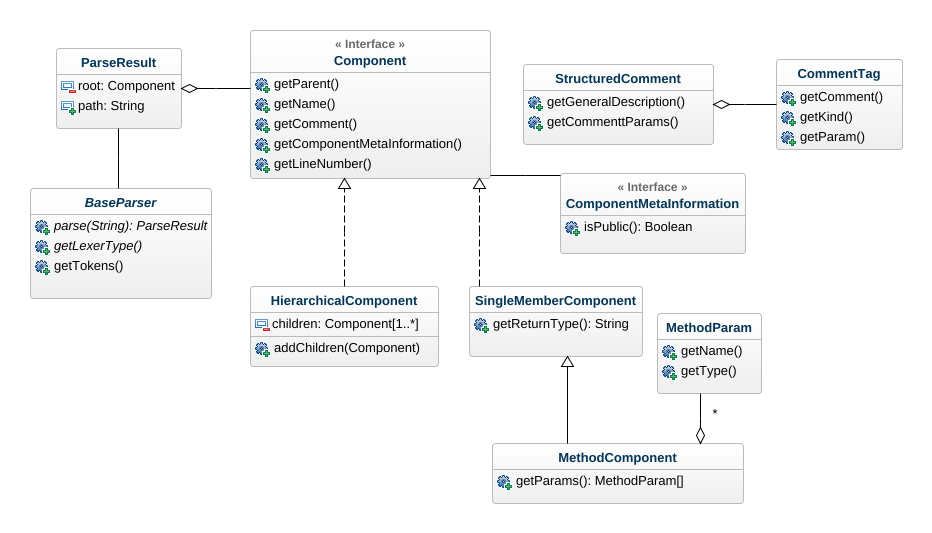
\includegraphics[width=\columnwidth]{figures/uml/parsing.png}
    \caption{UML-Diagramm mit allen wichtigen Klassen für das Parsen}
    \label{fig:uml_parsing}
\end{figure}

\subsubsection{ANTLR4}
Um die Java-Dateien zu parsen, wird die Bibliothek ANTLR4 verwendet, die kostenlos verfügbar ist. Diese Bibliothek kann nicht nur viele Programmiersprachen, sondern auch selbst geschriebene Sprachen parsen, sofern eine passende Grammatik verfügbar ist. Daneben gibt es noch Bibliotheken wie Bison, PEG.JS, die ebenfalls eine ähnliche Aufgabe erfüllen können. Allerdings gibt es bereits vordefinierte Grammatiken für ANTLR4, sodass ein erheblicher Aufwand gespart werden konnte.  

Zuvor wurde bereits versucht, die Java-Dateien mittels der NPM-Bibliothek \enquote{java-parser} \cite{Java-parser} zu parsen. Dies hätte den Vorteil, dass das Parsen, welches nicht der Hauptfokus dieser Bachelorarbeit ist, ausgelagert wird und so Fehler vermieden werden. Allerdings konnte diese Bibliothek nicht die Verbindung zwischen einer Komponente und der dazugehörigen Javadoc herstellen, sodass eine Benutzung dieser Bibliothek die Arbeit deutlich erschwert hätte. Daher fiel die Wahl auf \textit{ANTLR4}. Außerdem wurde zunächst versucht eine eigene Grammatik für Java zu schreiben, da die originale Grammatik für Java sämtliche Kommentare ignoriert. Da dies jedoch deutlich komplizierter war als erwartet, wurde dennoch entschieden, die von vielen Entwicklern geschriebene Grammatik zu verwenden (siehe unten).

\subsubsection{Lexer und Parser}
Eine Grammatik besteht immer aus einer Lexer-Grammatik und eine Parser-Grammatik, die jeweils vom Lexer bzw. Parser in dieser Reihenfolge verarbeitet werden, um so eine Baumstruktur einer Quellcodedatei zu erhalten. Der Lexer erstellt aus einer Quellcodedatei eine Liste von Tokens. Dabei ist ein Token eine Gruppierung von einem oder mehreren Zeichen, die eine weitergehende Bedeutung haben. Beispielsweise können Schlüsselwörter einer Programmiersprache oder Operatoren als Token klassifiziert werden. Diese Tokens sind grundsätzlich kontextunabhängig, das heißt für die gleiche Zeichenkette wird das gleiche Token verwendet. Jeder Token wird durch seine Zeichenkette und den Tokentyp klassifiziert

Quelltext \ref{lst:lexer_example} zeigt zur Verdeutlichung der Syntax eine Zeile aus der Lexer-Grammatik. 
		\begin{figure} [htbp]
			\lstinputlisting
			[caption={Beispielhafte Syntax vom Lexer},
			label={lst:lexer_example},
			captionpos=b, basicstyle=\footnotesize, tabsize=2, showstringspaces=false,  numbers=left]
			{figures/lexer_example.g4}
		\end{figure}

Eine Zeile in der Lexer-Grammatik beginnt mit den Namen eines Tokens, gefolgt von einem Doppelpunkt und dann einem regulären Ausdruck, der dieses Token beschreibt. Hier wird ein Javadoc-Kommentar definiert, das mit \enquote{/**} beginnt, dann folgen beliebige Zeichen und endet mit \enquote{*/}. Traditionell haben die Bezeichner der Tokens nur Großbuchstaben, sie müssen auf jeden Fall mit einem Großbuchstaben beginnen \cite[S. 3]{ANTLR:APredicated-<i>LLk</i>ParserGenerator}. 

Der nächste Schritt ist das eigentliche Parsen. Dabei werden die im vorherigen Schritt generierten Tokens, die als Liste vorliegen, genommen und in eine hierarchische Baumstruktur umgewandelt, wobei hier der Kontext die entscheidende Rolle spielt. ANTLR4 lädt ein Token nach dem anderen und prüft ob es, basierend auf der aktuellen Position in der Baumstruktur, eine Regel gibt, die durch diesen Token erfüllt wird. Wenn es mehrere mögliche Pfade gibt, lädt ANTLR4 so viele Tokens bis die nächste Regel eindeutig feststeht. Gibt es dennoch Uneindeutigkeiten, so wird die Regel genommen, die als erstes in Parser-Datei geschrieben wurde.

So kann eine vereinfachte Parser-Grammatik für Java einen Baumknoten definieren, der eine generelle Methode beschreibt. Eine Methode besteht nämlich aus Rückgabetyp, Bezeichner und Parameterliste. Die Parameterliste kann dann als eine Liste von Datentyp-Bezeichner-Paare aufgelöst werden. Der Rückgabetyp einer Methode ist allerdings anders zu verstehen als der Datentyp eines Parameters, da jeder Datentyp eines Parameters auch ein gültiger Rückgabetyp ist, was jedoch nicht umgekehrt der Fall ist; so ist \textit{}{void} ein gültiger Rückgabetyp, aber kein Datentyp. Quelltext \ref{lst:parser_example} zeigt ein typischer Ausschnitt aus einer Parser-Grammatik, wobei zur Übersichtlichkeit nicht alle Regeln und Tokens aufgelistet sind:
		\begin{figure} [htbp]
			\lstinputlisting
			[caption={Beispielhafte Syntax vom Parser},
			label={lst:parser_example},
			captionpos=b, basicstyle=\footnotesize, tabsize=2, showstringspaces=false,  numbers=left]
			{figures/parser_example.g4}
		\end{figure}
		
Der Ausschnitt beschreibt die notwendigen Regeln, um Methodenparameter zu parsen. Ein Methodenparameter kann keinen, einen oder mehrere  Modifizierer enthalten, die ihrerseits eine Java-Annotation sein können oder das Schlüsselwort\textit{final}. Anschließend muss ein Datentyp erfolgen, der wiederum aus einer Annotation bestehen kann, gefolgt von entweder einem primitiven Datentyp oder einem Klassen bzw. Schnittstellentyp. Auch die üblichen eckigen Klammern für Arrays in Java können nach diesem Datentyp folgen. Die letzte Voraussetzung für einen gültigen Methodenparameter ist ein valider Bezeichner.

Die Parser-Grammatik ist ähnlich wie die der Lexer-Grammatik aufgebaut. Auch hier wird eine Variante der regulären Ausdrücken verwende, wobei hier hier die reguläre Grammatik auf die Tokens (oder auf Zeichenketten, die eindeutig einem Token zugeordnet werden können) angewendet. Im Gegensatz zum Lexer muss der Bezeichner einer Parser-Regel mit einem Kleinbuchstaben beginnen\cite[S. 3]{ANTLR:APredicated-<i>LLk</i>ParserGenerator} \cite[S. 10ff.]{TheDefinitiveANTLR4Reference}. So ist eine Unterscheidung zwischen Tokens und den Parserregeln stets möglich. 


Basierend auf diese Baumstruktur des Parsers kann eine Quellcodedatei analysiert werden und so alle relevanten Informationen gesammelt werden. 
Dies lässt sich relativ leicht mit dem Visitor-Pattern erledigen, da so nur die relevanten  Komponenten genauer betrachtet werden müsse und alle uninteressanten Komponenten automatisiert durchlaufen werden, bis eine relevante Komponente gefunden wird. Quelltext \ref{lst:visit_method_example} zeigt einen Ausschnitt aus dem Java-Parser um das Visitor-Pattern genauer zu erläutern.

		\begin{figure} [htbp]
			\lstinputlisting
			[caption={Codeauschnitt aus  Methoden-Visitor},
			label={lst:visit_method_example},
			captionpos=b,language=java, basicstyle=\footnotesize, tabsize=2, showstringspaces=false,  numbers=left]
			{figures/visit_method_example.java}
		\end{figure}
Das Code-Snippet zeigt den einen Ausschnitt vom Visitor für Methodendeklarationen. Hier ist die Baumstruktur leicht sichtbar. Alle Einzelbestandteile einer Methode wie z. B. Bezeichner, Rückgabetyp etc. sind Kindknoten des \textit{RuleContext} und können über die Methode \textit{getChild} abgerufen werden. So werden sowohl der Bezeichner als auch der Rückgabetyp direkt als Text abgerufen. Theoretisch bestehen diese beiden Bestandteile auch aus weiteren Kindknoten, doch eine weitergehende Betrachtung ist nicht nötig, da nur die Bezeichnung als Zeichenkette benötigt wird. Andere Bestandteile wie die Methodenparameter sind jedoch komplexer, aus diesem Grund werden sie von separaten Visitors betrachtet.

\subsubsection{Implementierung von ANTLR4}
Für die Programmiersprache Java steht bereits eine Grammatik, die auf Github unter der BSD-Lizenz angeboten wird ist, zur Verfügung\cite{antlr_grammar_github}, allerdings ignoriert sie die Kommentare. Daher mussten einige Änderungen sowohl am Lexer als auch am Parser vorgenommen werden. Im Lexer werden standardmäßig alle Tokens in einem Kommentar in einen versteckten Kanal gespeichert, was dazu führt, dass diese Tokens vom Parser ignoriert werden. Daher wurde dieses Verhalten durch Definition eines neuen Tokens so geändert, dass Javadoc-Kommentare auch vom Parser verarbeitet werden können, aber mehrzeilige und einzeilige Kommentare weiterhin ignoriert werden. Einzeilige Kommentare sind hier nicht relevant, da sie kein Javadoc enthalten. Mehrzeilige Kommentare könnten theoretisch auch berücksichtigt werden, da einige Entwickler diese anstelle von Javadoc benutzen. Allerdings werden solche mehrzeilige Kommentare vor Komponenten nicht von Tools erkannt und haben daher einen geringeren, aber durchaus vorhandenen Nutzen \cite[S. 4]{HowDocumentationEvolvesoverTime}.

Deshalb wurde entschieden, Komponenten, die zwar mit mehrzeiligen Kommentaren aber nicht mit Javadoc dokumentiert sind, wie undokumentierte Komponenten zu betrachten. Für einen Entwickler sollte es so schnell möglich sein, solche nicht korrekt dokumentierten Komponenten zu identifizieren und deren mehrzeilige Kommentare in gültige Javadoc-Kommentare umzuwandeln und so die Qualität der Dokumentation zu erhöhen. Für andere Programmiersprachen können jedoch normale mehrzeilige wie strukturierte Kommentare betrachtet werden, wenn dies für sinnvollerer erachtet wird.

Mehr Änderungen mussten an der entsprechenden Parser-Datei \textit{JavaParser.g4} durchgeführt werden.  Tabelle \ref{tab:parser_changes} listet alle Änderungen an der Parserdatei auf;
\begin{table}[h!]
    \centering
    \begin{tabular}{m{0.75cm}|m{4cm}|m{10cm}}
        Zeile & Änderung & Begründung \\
         \hline
        116 & Deklaration Kommentar & Hier wird ein mehrzeiliger Kommentar definiert, dies ist hier ein Alias für den Token \textit{JCOMMENT}\\
        \hline
        128 & \textit{comment} als möglicher Präfix in Klassenmember & Hier wird dem Parser mitgeteilt, dass ein Bestandteil einer Klasse wie z. B. eine Methode einen Javadoc-Kommentar besitzen kann\\
        \hline
        47 & \textit{comment} als möglicher Präfix vor Datentyp & Hier wird dem Parser mitgeteilt, dass ein Datentyp (Klasse, Schnittstelle etc. ) einen Javadoc-Kommentar haben kann \\
        \hline
        404 & Zulassung von Javadoc in Methoden & Da Javadoc-Kommentare an beliebigen Stellen auftauchen können, auch wenn es nicht empfohlen wird und keinen Mehrwert bietet, wird hier sichergestellt, dass solche Kommentare nicht zu Warnungen oder Fehler von ANTLR4 führen. Diese Javadoc-Kommentare werden nichtsdestotrotz später ignoriert.\\
        \hline
        34, 38& Zulassung von Kommentaren vor Paketdeklarationen und Imports & Hier werden Kommentare auch vor Paketdeklarationen und Import-Statements erlaubt, was vor allem bei Klassen mit Urheberrechtsangabe sinnvoll ist\\
        \hline
        105 & Zulassung von Kommentaren bei Enumerationen & Zwar werden Javadoc-Kommentare in Enumerationen mit diesem Tool nicht betrachtet, sie führen aber dennoch zu Warnungen und Fehlermeldungen. Daher werden sie hier zugelassen, aber später ignoriert. \\
        \hline
        82, 83 & Erzeugung eines separaten Knotens für \textit{Extends}- und \textit{Implements}-Deklarationen & In der originalen Version der Parserdatei wurde die Definition der Basisklasse bzw. der implementierten Schnittstellen direkt über die Tokens \textit{EXTENDS} bzw. \textit{IMPLEMENTS} gelöst. Dies wurde in einem neuen Knoten \textit{extendClass} bzw. \textit{implementInterfaces} ausgegliedert, um so das Parsing etwas zu vereinfachen.  \\
         \hline
    \end{tabular}
    \caption{Änderungen an der Parserdatei}
    \label{tab:parser_changes}
\end{table}

\subsection{Metriken anwenden}
\begin{figure}
    \centering
    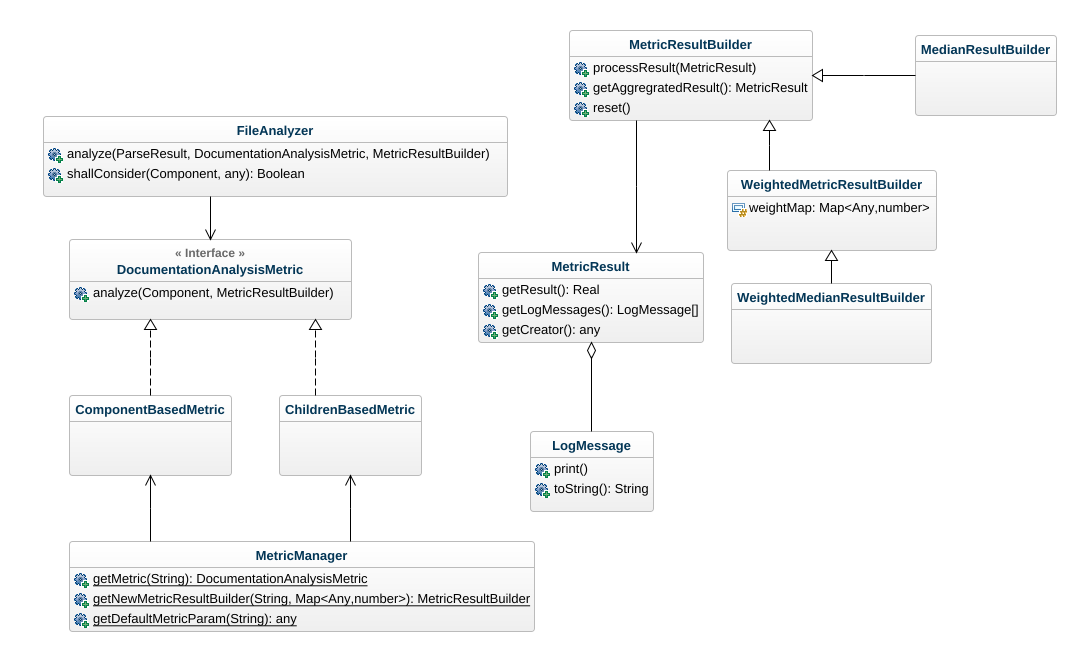
\includegraphics[width=\columnwidth]{figures/uml/metriken.png}
    \caption{UML-Diagramme aller Klassen, die relevant für die Metriken sind}
    \label{fig:uml_metrics}
\end{figure}
Als nächster Schritt müssen auf die Informationen bezüglich der Dokumentation, die der Parser im vorherigen Schritt gesammelt hat, geeignet ausgewertet werden. Dazu können verschiedene Metriken verwenden, die im Späteren genauer erläutert werden. Dabei gibt es genau zwei Kategorien an Metriken. Die meisten Metriken arbeiten nur auf eine Komponente und der dazugehörigen Dokumentation. Andere Metriken sind nur mit hierarchischen Komponenten kompatibel und analysieren die Kommentare all ihrer Kinder. 

Jede Metrik gibt eine numerische Bewertung ab, die eine Aussage über die Dokumentationsqualität trifft. Hier wurde eine 0 für sehr schlechte bis nicht existente Dokumentation und 100 für eine exzellente Dokumentation gewählt, sodass die Bewertung sich als Prozent lesen lassen kann. Grundsätzlich ist aber auch ein anderer Wertebereich möglich. Eine Metrik kann sich aber auch dafür entscheiden, eine Komponente komplett zu ignorieren, sodass sie für diese Metrik als nicht existent betrachtet wird.

Zudem können Metriken Warn- oder Fehlermeldungen werfen, um den Anwender des Programms auf schlechte Dokumentation aufmerksam zu machen. Diese Fehlermeldung enthalten auch den Komponentennamen und die Zeilennummern, damit der Programmierer schnell auf die verwendete Komponente zugreifen kann.\bigskip
\subsection{Resultate der Metriken anwenden}
Da in einer Datei mehrere Komponenten durchaus Standard sind, müssen die Bewertungen jeder Komponente passend aggregiert werden. Dazu wurde ein \textit{MetricResultBuilder} entwickelt. Dieser kann durch die Methode \textit{processResult} das Resultat einer Metrik verarbeiten, indem es sie in einer Liste speichert. Wenn alle Metriken verarbeitet sind, muss daraus ein Gesamtresultat gebildet werden. Dies geschieht durch die Methode \textit{getAggregratedResult}. Dabei wird standardmäßig ein einfacher arithmetischer Mittelwert gebildet. Es sind auch aber auch andere \enquote{ResultBuilder} standardmäßig implementiert, sodass der Benutzer des Tools einen geeigneten Algorithmus auswählen kann. Ein \textit{ResultBuilder} wurde nach dem Vorbild des Design-Patterns \enquote{Builder} aus \cite[S.139-149]{gamma2015design} entwickelt, da es aus einzelnen Metrikresultaten ein vollständiges Metrikergebnis baut. 

In den folgenden Unterabschnitten wird jeder Algorithmus kurz erläutert und dabei kurz auf die Vor- und Nachteile eingegangen. Auch werden die möglichen Aliasnamen angegeben, mit der der Algorithmus in der Konfigurationsdatei angesprochen werden kann. 

\subsubsection{Einfacher Mittelwert}
Der einfache arithmetische Mittelwert wird bereits durch die Klasse \textit{MetricResultBuilder} implementiert. Er summiert die Ergebnisse auf und teilt diese durch die Anzahl der Einzelresultate. Dieser Algorithmus ist einfach zu verstehen und berücksichtigt jedes Ergebnis gleichermaßen. Dies ist insbesondere für die Aggregierung der Ergebnisse der einzelnen Dateien sinnvoll, da jede Datei gleich behandelt werden sollte und eine Gewichtung von möglicherweise Tausenden von Dateien nur schwer umsetzbar ist. Es sollte allerdings auch beachtet werden, dass der Mittelwert extreme Ausreißer berücksichtigt. Dies ist hier manchmal sinnvoll, da sehr schlechte oder sehr gute Dokumentation besser berücksichtigt wird und so ein verlässliches Gesamtergebnis geliefert wird.


\subsubsection{Median}
Der Median der Einzelresultate wird von der Klasse \textit{MedianResultBuilder} berechnet. Dabei werden die Einzelresultate nach ihrem Gewicht sortiert und dann das Resultat genommen, das in der sortierten Liste in der Mitte liegt. Bei einer geraden Anzahl an Elementen wird der Median aus dem Mittelwert der zwei infrage kommenden Ergebnissen gebildet. 

Der Median berücksichtigt extreme Ausreißer nicht und kann daher interessant sein, wenn ein allgemeines Bild von der Dokumentationsqualität gemacht werden soll. Es sollte aber beachtet werden, dass die Anwendung des Medians ein Sortiervorgang benötigt, der mindestens eine Komplexität von $O(n*log(n)$ hat. Bei der überschaubaren Anzahl an Metriken wird dies nicht so relevant sein, bei einer Anwendung des Medians auf vielen Dateien durchaus wohl.


\subsubsection{Gewichteter Mittelwert}
Der gewichtete Mittelwert ist in der Klasse \textit{WeightedMetricResultBuilder} implementiert. Dabei wird dem Konstruktor dieser Klasse eine assoziative Liste übergeben, die einem Metrikobjekt ein Gewicht zuordnet.  Es wird dabei davon ausgegangen, dass jede Metrik nur von einer Instanz repräsentiert wird. Dies ist nur möglich, da die Metriken keinen inneren Zustand haben und nur mittels lokale Variablen und Parameter arbeiten. Jedes Einzelresultat speichert zudem den Erzeuger des Ergebnisses, sodass für jede Metrik ein Gewicht abgerufen werden kann. Die Gewichte müssen nicht normiert werden, da dies während der Berechnung implizit gemacht wird. Die Resultate jeder Metrik werden multipliziert mit dessen Gewicht aufsummiert und dann durch die Summe aller Gewichte geteilt. 


Dieser Algorithmus ermöglicht es, bestimmte Metriken zu bevorzugen bzw. zu benachteiligen. Dies ist sinnvoll, da nicht jede Metrik immer ein aussagekräftiges Ergebnis liefert und bestimmte Metriken je nach Situation ein besseres Bild über die Dokumentationsqualität liefern. Allerdings ist auch zu beachten, dass die Wahl der Gewichte nicht trivial ist und ein Vergleich von Ergebnissen, die verschiedene Gewichte verwenden, nur selten sinnvoll ist.

\subsubsection{Gewichteter Median}
Der gewichtete Median wurde leicht abweichend nach \cite[S. 37]{YAGER199835} implementiert. Dabei wird zunächst die Summe der Gewichte berechnet und die Resultate nach ihrem Gewicht sortiert. Anschließend werden die sortierten Resultate und ihre Gewichte so lange aufsummiert, bis diese temporäre Summe die Hälfte der Gesamtsumme überschreitet. Das Metrikergebnis, bei der diese Bedingung zutrifft, ist das gesuchte Gesamtergebnis. Die Vor- und Nachteile dieses Algorithmus entsprechen in etwa den Vor- und Nachteilen des gewichteten Mittelwerts und des Medians. So muss auch hier eine Sortierung durchgeführt werden und die Wahl der richtigen Gewichte ist nicht trivial. 



\section{Konfiguration und Nutzung des Tools}
Das Tool benötigt einen Parameter, der das Verzeichnis angibt, das analysiert werden soll. Fehlt dieser Parameter wird eine Warnmeldung ausgegeben und das Tool nutzt das aktuelle Arbeitsverzeichnis. Die Konfigurationsdatei muss den Namen \enquote{comment\_conf.json} tragen. Als Alternative können auch Umgebungsvariablen über Github Actions gesetzt werden, wobei die Parameternamen dieselben sind. Ist sowohl in der Konfigurationsdatei als auch in der Umgebungsvariable eine Einstellung definiert, hat die Umgebungsvariable Vorrang, da das Tool für primär für Github Actions programmiert wurde.
\begin{table}[h]
    \centering
    \begin{tabular}{m{4cm}|m{11cm}}
    \hline
        Parameter & Beschreibung  \\
        \hline
        include & Alle Dateien, die bei der Bewertung der Dokumentationsqualität berücksichtigt werden müssen\\
        \hline
        Exclude & Teilmenge von include, enthält Dateien, die nicht weiter betrachtet werden müssen\\
        \hline
        metrics & Alle Metriken, die das Tool verwenden soll. Dies ist ein Array von Objekten mit der Strukur \enquote{(name,weight,params)}, wobei \textit{weight} das Gewicht der jeweiligen Metrik ist( Bei Algorithmen ohne Relevanz des Gewichts wird es ignoriert), \textit{name} der Name (oder Aliasname) der Metrik und \textit{params} ein Objekt mit den Parametern der Metrik\\\hline
        global\_threshold & Mindestwert der Bewertung ,der erreicht werden muss, sonst wird die Dokumentationsqualität nicht akzeptiert\\\hline
        metric\_result\_builder & Der Algorithmus/\textit{ResultBuilder}, der die einzelnen Ergebnisse der Metriken verarbeitet und so das Gesamtergebnis berechnet.\\\hline
          single\_file\_result\_builder & Der Algorithmus/\textit{ResultBuilder}, der die einzelnen Ergebnisse einer Datei verarbeitet\\\hline
        files\_result\_builder & Der Algorithmus/\textit{ResultBuilder}, der die einzelnen Ergebnisse aller Dateien verarbeitet
        
    \end{tabular}
    \caption{Parameter zur Konfiguration des Tools}
    \label{tab:tool_javadoc_conf}
\end{table}

\subsection{Einbindung in GitHub Actions}
Um das Tool in GitHub Actions einzubinden, mussten einige Schritte erfolgen. Zunächst musste eine \enquote{action.yaml} geschrieben werden, die das GitHub-Repository als Aktion markiert und die notwendige Befehle für die Ausführung enthält. Quelltext  \ref{lst:action} zeigt den kompletten Code der Aktion:
\begin{figure} [htbp]
\lstinputlisting
[caption={Action-Datei für das Tool},
label={lst:action},
captionpos=b, basicstyle=\footnotesize, tabsize=2, showstringspaces=false,  numbers=left]
{figures/action.yml}
\end{figure}

In den ersten beiden Zeilen werden triviale Attribute wie der Name und eine Beschreibung gesetzt. Danach wird der Eingabeparameter für die minimal erlaubte Bewertung für die Dokumentationsqualität definiert, damit dieser von den Nutzern der Aktion verändert werden kann.  Außerdem werden noch ein Icon und eine Farbe gesetzt, was aber hier nicht von Interesse ist. Die letzten Zeilen sind allerdings wichtig. Hier wird die Aktion als JavaScript-Aktion mit der Node-Version 16 festgelegt. Zudem enthält die letzte Zeile auch den Pfad zur Quellcodedatei, mit dem das Programm gestartet werden soll. 

Da das Programm in TypeScript programmiert wurde, eine JavaScript-Aktion aber reines JavaScript benötigt, sind weitere Schritte nötig. Es wurde ein weiterer Worklfow erstellt, der bei jedem Push in dem Main-Zweig folgende Schritte ausführt:
\begin{enumerate}
    \item Klonen der Main-Branch des Repositories(wie bei den meisten anderen Workflows)
    \item Aufruf von TSC, Konvertierung des TypeScript-Codes in JavaScript
    \item Aufruf und Benutzung von NCC\cite{ncc}. Packen aller JavaScript-Dateien in eine einzige Datei
    \item Kopieren der generierten Datei, die den gesamten Quellcode enthält und der \enquote{action.yml}, in eine (neue) Branch \textit{action}. Dies wird mittels der Aktion \textit{Branch-Push}\cite{Branch-Push} durchgeführt
\end{enumerate}
Durch diese Schritte wird eine neue Branch erstellt, die nur die notwendige JavaScript-Datei und die \textit{action.yml} enthält. Dadurch können Nutzer der Aktion diese schneller herunterladen und nutzen. Es wäre auch möglich, kein \enquote{NCC} zu verwenden, also alle Javascript-Dateien in die neue Branch zu kopieren, allerdings ist die hier gewählte Methode praktikabler,da dann nur ein Lesezugriff beim Starten des Programms erforderlich ist und so ein Geschwindigkeitsvorteil existiert. 

\subsubsection{Nutzung der Aktion}

Die oben erstellte Aktion kann nun von jedem GitHub-Repository verwendet werden. dazu kann der folgende Quelltext \ref{lst:action_using} als zusätzlicher Schritt in einem Workflow eingebunden werden. 
\begin{figure} [htbp]
\lstinputlisting
[caption={Verwendung der Aktion in einem Workflow},
label={lst:action_using},
captionpos=b, basicstyle=\footnotesize, tabsize=2, showstringspaces=false,  numbers=left]
{figures/action_using.yml}
\end{figure}

Hier wird die aktuelle Version des JavadocEvaluators aus der Branch \textit{action} heruntergeladen und automatisch ausgeführt. Als Parameter wird beispielsweise ein Grenzwert von 20 übergeben, der jedoch nach Belieben angepasst werden kann. Wenn das entsprechende Ereignis des Workflow eintritt (z. B. ein Push-Ereignis), wird der JavadocEvaluator mit dem Parameter aufgerufen und zeigt unter der Registerkarte \textit{Actions} eine Fehlermeldung an, wenn die Dokumentationsqualität den Grenzwert unterschreitet und somit nicht ausreichend ist. 